\documentclass[10pt]{article}
\usepackage[polish]{babel}
\usepackage[utf8]{inputenc}
\usepackage[T1]{fontenc}
\usepackage{amsmath}
\usepackage{amsfonts}
\usepackage{amssymb}
\usepackage[version=4]{mhchem}
\usepackage{stmaryrd}
\usepackage{graphicx}
\usepackage[export]{adjustbox}
\graphicspath{ {./images/} }

\title{XII Konkurs matematyczny St@ś }

\author{}
\date{}


\begin{document}
\maketitle
XIV LO im. Stanisława Staszica\\
4 czerwca 2012 roku

\section*{klasa VI}
Na rozwiqzanie poniższych zadań masz 90 minut. Kolejność rozwiazywania tych zadań jest dowolna. Wszystkie zadania sa jednakowo punktowane. Maksymalna liczbę punktów mȯ̇e uzyskać jedynie petne rozwiqzanie, z uzasadnieniem i odpowiedzia.\\
Używanie korektora i korzystanie z kalkulatora jest niedozwolone.

\begin{enumerate}
  \item Gdy Staś liczył cukierki układając je kupkami po cztery, zostały mu w ręku dwa. Gdy grupował je po pięć, to został mu jeden. Ile mógł ich mieć wiedząc, że liczba cukierków była dwucyfrowa. Odpowiedź uzasadnij.
  \item Tę samą dwucyfrową, liczbę całkowitą, dodatnią napisano trzy razy obok siebie. Czy uzyskana w ten sposób liczba sześciocyfrowa dzieli się przez\\
(a) 7\\
(b) 4 ?
  \item Wyznacz ostatnią cyfrę liczby
\end{enumerate}

\[
2^{1000}+4^{199}
\]

\begin{enumerate}
  \setcounter{enumi}{3}
  \item Do narysowania wielokąta wypukłego wraz z jego wszystkimi przekątnymi potrzebowano 45 odcinków. Ile boków ma ten wielokąt?
  \item Z jednego wierzchołka sześcianu poprowadzono dwie przekątne jego dwóch ścian, tak jak na rysunku. Wyznacz miarę kąta między tymi przekątnymi. Narysuj siatkę tego sześcianu.\\
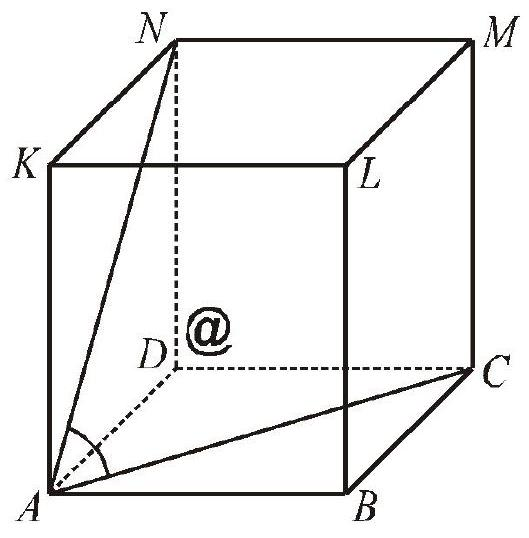
\includegraphics[max width=\textwidth, center]{2024_11_21_ddff019caeba361186e5g-1}
\end{enumerate}

\end{document}